\documentclass{article}
\usepackage[utf8]{inputenc}
\usepackage[margin = 1in]{geometry}
\usepackage{multicol}
\setlength{\columnsep}{.4in}

\usepackage{graphicx} %package to manage images
\graphicspath{ {./Images/} }

\title{Leap Frogging Vortices}
\author{Nathan Mortensen}
\date{December 2021}

\begin{document}

\maketitle
\tableofcontents
\pagebreak
\begin{multicols}{2}
\section{Introduction}

Vortex rings are caused when a fluid is forced through a hole, which causes the fluid to turn back in on itself and create ring. As the velocity of a vortex ring decreases, the vortex ring expands in size, eventually causing the vortex ring to disappear. However, the life of a vortex ring can be prolonged with the addition of a second ring. If set up properly, the interaction between the rings can cause them to propel the other forward, or "leap frog." This process causes the diameter of the rings to fluctuate in size.
This paper will analyze the interaction of two vortex rings in a two dimensional space, idealized as four vertices in a square layout (see figure 1).

\begin{center}
\includegraphics{Vortex Layout}

\caption{Figure 1: The cross section of two vortex rings, identified by four vertices. The vertices are labeled as follows, starting with the bottom left and going around counter clockwise, 1, 2, 3, and 4.}
\end{center}

\section{Methodology}
The unit vector form of the vortex velocity equation is as follows
\begin{equation}
   \vec{V} = \frac{\vec{\Gamma} \times \hat{r}}{2\pi r}
\end{equation}
Where gamma denotes the strength of the vortex, the unit vector denotes the direction of the vortex that is inducing the velocity on the vortex being analyzed, and r is a scalar value of that distance.
Making note that the unit vector can be rewritten as

\begin{equation}
\hat{r} = \frac{\vec{r}}{|\vec{r}|}
\end{equation}

the vortex velocity equation can be rewritten as

\begin{equation}
\vec{V} = \frac{\vec{\Gamma} \times \vec{r}}{2\pi r^2}
\end{equation}

In order to resolve this equation so it can be used for multiple vortex rings, it is necessary to note that

\begin{equation}
\vec{V}_t_o_t = \sum \vec{V}
\end{equation}

and that clockwise vertices enact a positive velocity on the vortex being analyzed, while counterclockwise vertices induce a negative velocity on the same ring. This leads to the velocity equation for each vortex in the two vortex example being

\begin{equation}
\vec{V_1} = \vec{V}_1_t_o_4 - \vec{V}_1_t_o_2 - \vec{V}_1_t_o_3
\end{equation}

\begin{equation}
\vec{V_2} = \vec{V}_2_t_o_4 + \vec{V}_2_t_o_1 - \vec{V}_2_t_o_3
\end{equation}

\begin{equation}
\vec{V_3} = \vec{V}_3_t_o_4 + \vec{V}_3_t_o_1 - \vec{V}_3_t_o_1
\end{equation}

\begin{equation}
\vec{V_4} = \vec{V}_4_t_o_1 - \vec{V}_4_t_o_2 - \vec{V}_4_t_o_3
\end{equation}

By using basic kinematics in conjunction with a time step, it is possible to estimate the new position of each vortex.

\begin{equation}
\vec{P}_f = \vec{P}_i +\vec{V}dt
\end{equation}

In order to continue estimating the velocity and location of each of the vertices, repeat the previous process.

\section{Results}
Figure 2 shows the varying size of each vortex ring as they move along the horizontal access. As long as the time step has an adequate resolution, this pattern will repeat indefinitely in an inviscid fluid. However, in real life the frictional force that the fluid's viscosity imparts on the vortex rings will cause them to slow down and eventually dissipate.
\begin{center}

\resizebox{7cm}{!} {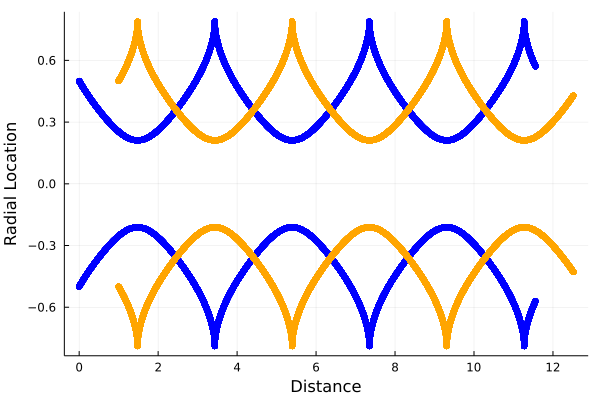
\includegraphics{Images/LeapFrog.png}}

\caption{Figure 2: Position graph of leap frogging vortex rings with a circulation of [0,0,1], initial separation distance of 1 unit, time step of .001 seconds, and time duration of 40 seconds}
\end{center}

Increasing the magnitude of the circulation vector has a direct impact on the velocity of the vortex rings, which shortens the distance of each cycle on the position graph, as seen in figure 3. It also increases the distance traveled, as the rings in figure 3 traveled approximately twice the distance as the rings in figure 2 in a fifth of the time.

\begin{center}

\resizebox{7cm}{!} {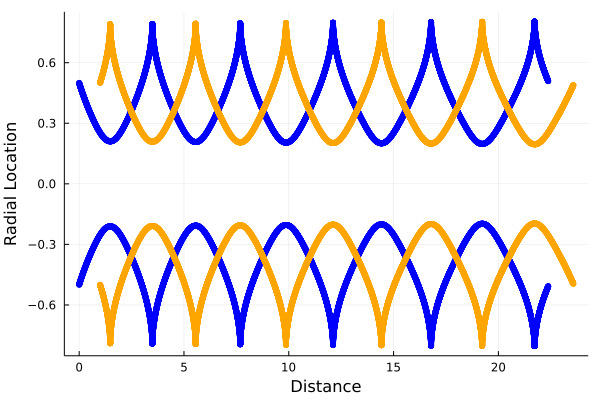
\includegraphics{Images/LeapFrog[0,0,10].png}}

\caption{Figure 3: Position graph of leap frogging vortex rings with a circulation of [0,0,10], initial separation distance of 1 unit, time step of .001 seconds, and time duration of 8 seconds}
\end{center}

Lastly, changing the distance between the vertices has a inverse relationship with the velocity of the rings, as shown in figure 4. The increased distance greatly decreases the impact that the surrounding vertices have on each other. This impact could be mitigated by having two separate variables for the initial distance separating the vortex rings and the initial diameter of the vortex rings. This would allow the additional analysis of large vortex rings close together and small vortex rings that are far apart.


\begin{center}
\resizebox{7cm}{!} {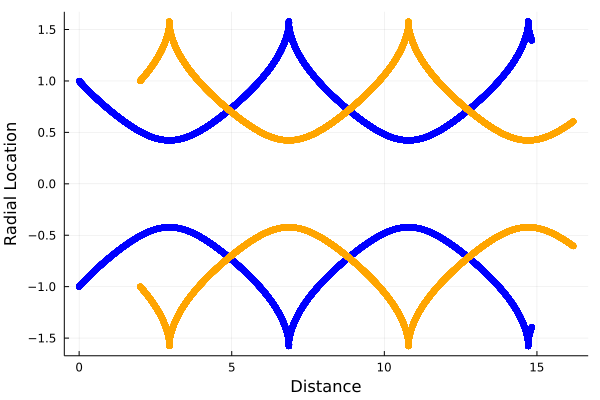
\includegraphics{Images/LeapFrogd2.png}}

\caption{Figure 4: Position graph of leap frogging vortex rings with a circulation of [0,0,1], initial separation distance of 2 units, time step of .001 seconds, and time duration of 100 seconds}
\end{center}


\end{multicols}
\end{document}
